\documentclass[11pt, a4paper,twocolumn]{jarticle}
\usepackage[dvipdfmx]{graphicx}
\usepackage{listings,jlisting}

\begin{document}
%=============================================================
\section{Comparison between tow- and four-terminal measurements($1^{st} day$)}

\subsection{Purpose}
低抵抗サンプルを4端子測定法と2端子測定法によって抵抗測定をしてその違いについて考える.
\subsection{Procedure}
抵抗(10Ω,50Ω,1kΩ)と直径の異なる二つの銅線(0.1mm,0.122mm)に電流を流し電圧計,電流計を用いて4端子測定法,2端子測定法によりその抵抗を測定をし,その違いについて考える.

また金属の抵抗値,抵抗率の関係は以下の数式によって定義されている.

\begin{equation}
    R = \rho\frac{l}{S}(\Omega)
\end{equation}

この関係式に今回の実験条件の(l = 1cm),断面積S,測定抵抗Rを代入する事により銅の抵抗率を求めた.
また4端子測定法,2端子測定法はサンプルに対して以下のように計測器をつなぐ.

\begin{figure}[htbp]
 \begin{center}
  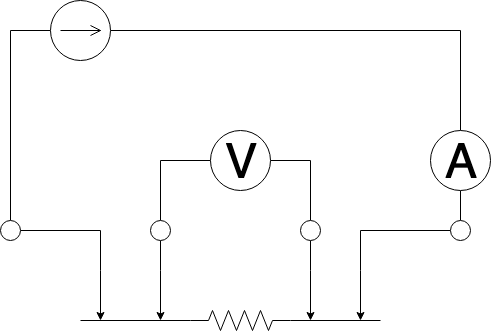
\includegraphics[width=0.8\linewidth]{fig1.png}
 \end{center}
 \caption{4端子測定法}
 \label{fig:1}
\end{figure}
\newpage
\begin{figure}[htbp]
 \begin{center}
  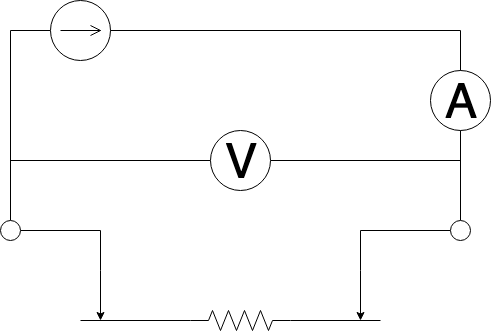
\includegraphics[width=0.8\linewidth]{fig2.png}
 \end{center}
 \caption{2端子測定法}
 \label{fig:2}
\end{figure}

\subsection{Result}
測定の結果電流電圧の関係をプロットすると以下のようなグラフが得られた.

\begin{figure}[htbp]
 \begin{center}
  \includegraphics[width=0.8\linewidth]{fig4.png}
 \end{center}
 \caption{4端子10$\Omega$}
 \label{fig:4}
\end{figure}

\begin{figure}[htbp]
 \begin{center}
  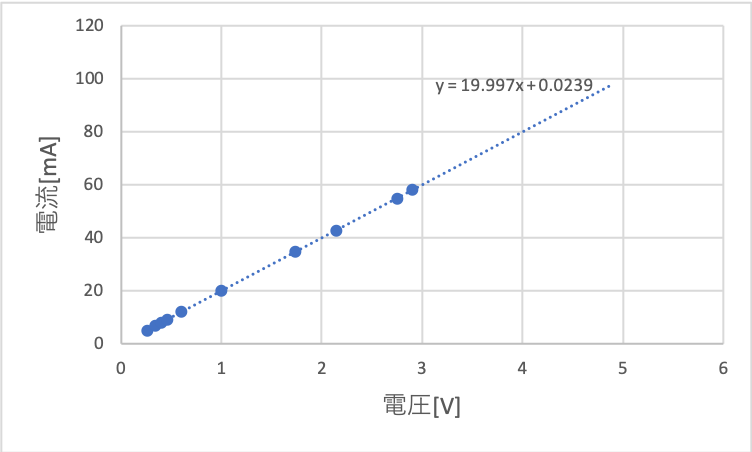
\includegraphics[width=0.8\linewidth]{fig3.png}
 \end{center}
 \caption{4端子50$\Omega$}
 \label{fig:3}
\end{figure}

\begin{figure}[htbp]
 \begin{center}
  \includegraphics[width=0.8\linewidth]{fig5.png}
 \end{center}
 \caption{4端子1k$\Omega$}
 \label{fig:5}
\end{figure}

\begin{figure}[htbp]
 \begin{center}
  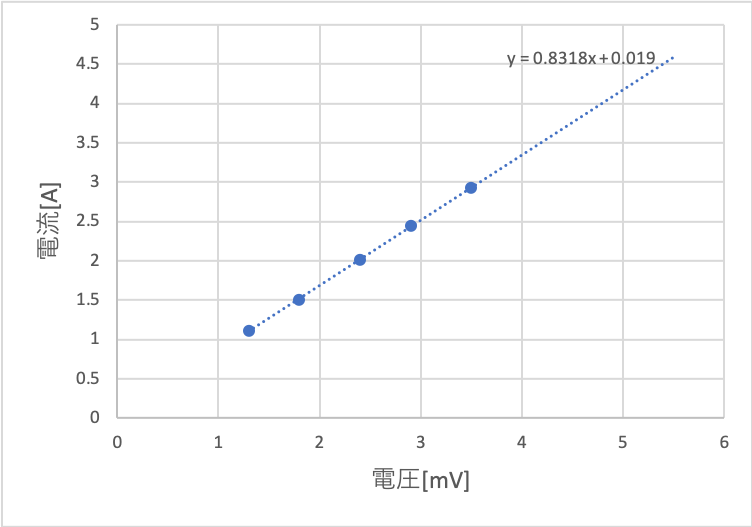
\includegraphics[width=0.8\linewidth]{fig6.png}
 \end{center}
 \caption{4端子0.1mm銅線}
 \label{fig:6}
\end{figure}

\begin{figure}[htbp]
 \begin{center}
  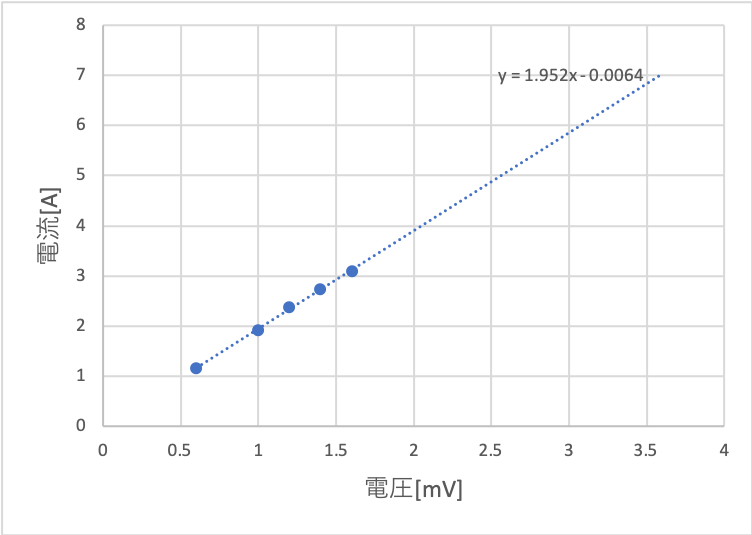
\includegraphics[width=0.8\linewidth]{fig7.png}
 \end{center}
 \caption{4端子0.122mm銅線}
 \label{fig:7}
\end{figure}

\begin{figure}[htbp]
 \begin{center}
  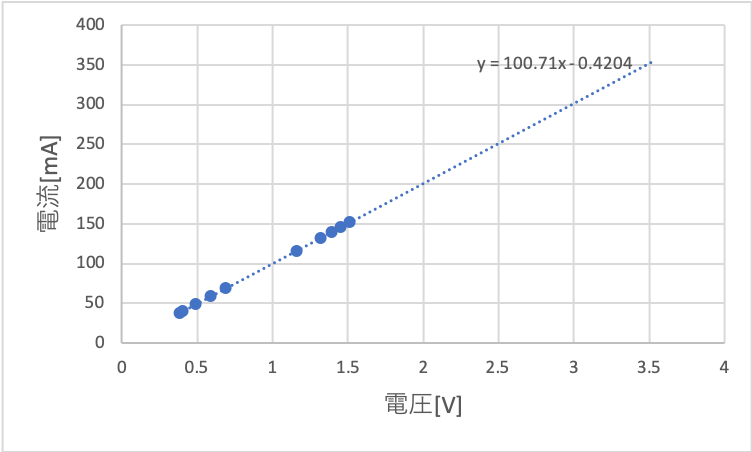
\includegraphics[width=0.8\linewidth]{fig9.png}
 \end{center}
 \caption{2端子10$\Omega$}
 \label{fig:9}
\end{figure}

\begin{figure}[htbp]
 \begin{center}
  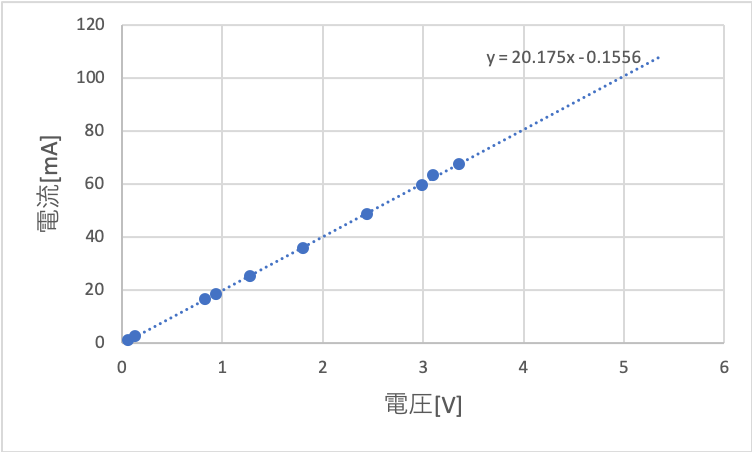
\includegraphics[width=0.8\linewidth]{fig8.png}
 \end{center}
 \caption{2端子50$\Omega$}
 \label{fig:8}
\end{figure}

\begin{figure}[htbp]
 \begin{center}
  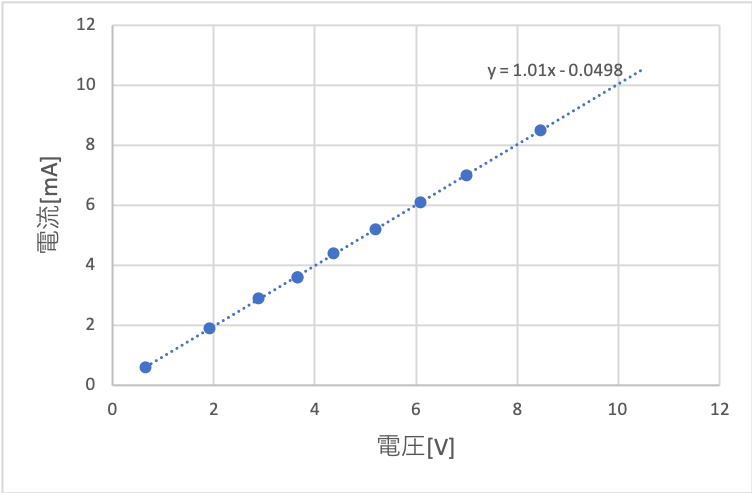
\includegraphics[width=0.8\linewidth]{fig10.png}
 \end{center}
 \caption{2端子1k$\Omega$}
 \label{fig:10}
\end{figure}

\begin{figure}[htbp]
 \begin{center}
  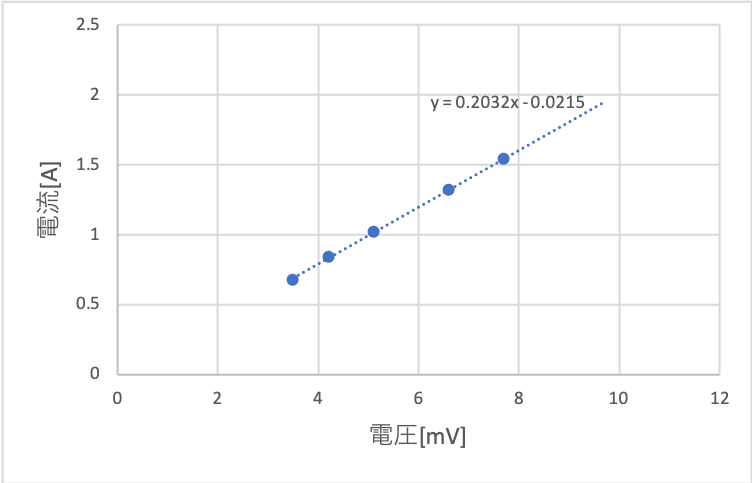
\includegraphics[width=0.8\linewidth]{fig11.png}
 \end{center}
 \caption{2端子0.1mm銅線}
 \label{fig:11}
\end{figure}

\begin{figure}[htbp]
 \begin{center}
  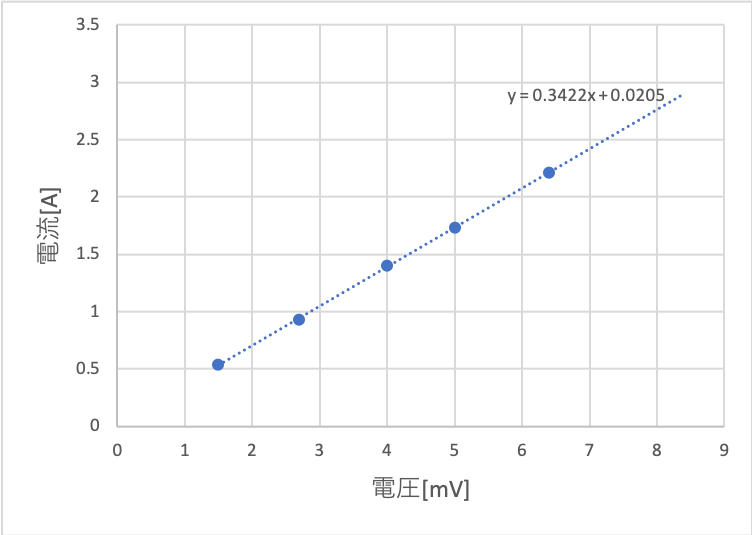
\includegraphics[width=0.8\linewidth]{fig12.png}
 \end{center}
 \caption{2端子0.122mm銅線}
 \label{fig:12}
\end{figure}
\newpage
以上の結果よりグラフの傾きを最小二乗法によって求めそれぞれの抵抗値を求めたところ表\ref{tab:1}のようになった.

またそれぞれの場合において抵抗率は表\ref{tab:2}のようになった.

\begin{table}[htb]
  \begin{center}
      \caption{抵抗値($\Omega$)}
        \begin{tabular}{|c|c|c|} \hline
              & 4端子 & 2端子 \\ \hline
          10$\Omega$ & 9.821 & 9.930  \\
          50$\Omega$ & 50.01 & 49.57 \\
          1k$\Omega$ & 987.8 & 990.1 \\
          0.1mm銅線   & 0.001202 & 4921 \\
          0.122mm銅線 & 0.0005123 & 2922 \\ \hline
        \end{tabular}
        \label{tab:1}
  \end{center}
\end{table}

\begin{table}[htb]
  \begin{center}
      \caption{抵抗値($\mu\Omega$cm)}
        \begin{tabular}{|c|c|c|} \hline
              & 4端子 & 2端子 \\ \hline
          0.1mm銅線   & 0.0944 & 0.387 \\
          0.122mm銅線 & 0.0599 & 0.342 \\ \hline
        \end{tabular}
        \label{tab:2}
  \end{center}
\end{table}



\subsection{Discussion}
まず四端子測定法と二端子測定法の違いについて考察する.
図\ref{fig:13},図\ref{fig:14}にそれぞれの回路図を示す.
ここでRAは電流計の内部抵抗,Rsはサンプル抵抗,r1,r2,r3,r4は測定回路における接触抵抗およびリード線の抵抗とする.
また電圧計の内部抵抗は十分に大きいものとして抵抗値無限大を考える.

\noindent
二端子測定法の場合

この時電流計の内部抵抗RAの値は測定には影響を与えないため考慮しない事にする.
また電圧計の抵抗は無限大としているため電圧計に流れる電流は0とみなす.
すると測定電圧V,測定電流Aの関係は次のようになる.
\begin{equation}
    \frac{V}{I} = r1 + r2 + Rs
\end{equation}

\noindent
四端子測定法の場合

この時も同様に電圧計の内部抵抗は十分に大きいと言えるので電圧計に流れる電流は無視できる.すると測定電圧と測定電流の関係は次のように表せる.
\begin{equation}
    \frac{V}{I} = Rs
\end{equation}

以上の考察より二端子測定法ではサンプル抵抗と同様に余計な抵抗r3,r4を測定してしまうためサンプル抵抗が小さい場合の測定方法には適していないと考えられる.

接触抵抗およびリード線の抵抗が~100$\Omega$と考えれば10k$\Omega$より大きいサンプル抵抗を測定する際には誤差を1\%以内に抑えることができると予想される.

今回の場合は測定する抵抗値は比較的小さいので四端子測定法で測定する方が望ましいと考えられる.
また二端子測定法は四端子測定法に比べて余分な接触抵抗まで測定してしまうので四端子測定に比べて測定抵抗値が大きく表示されてしまうと考えられる.
実際表\ref{tab:1}においていずれの場合も二端子測定法で測定を行った方が抵抗値が高く測定されたのでこの考えは正しいと予想できる.


\begin{figure}[htbp]
 \begin{center}
  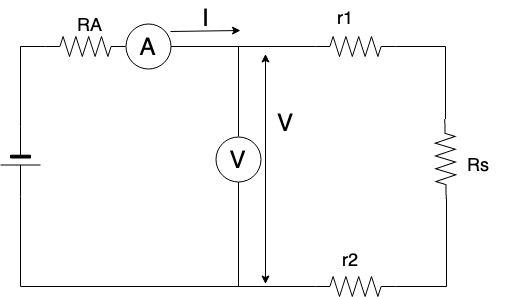
\includegraphics[width=0.8\linewidth]{fig13.png}
 \end{center}
 \caption{二端子測定法}
 \label{fig:13}
\end{figure}

\begin{figure}[htbp]
 \begin{center}
  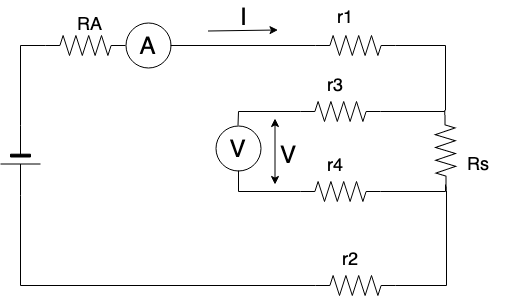
\includegraphics[width=0.8\linewidth]{fig14.png}
 \end{center}
 \caption{四端子測定法}
 \label{fig:14}
\end{figure}
%=============================================================
\newpage
\end{document}
